%%%%%%%%%%%%%%%%%%%%%%%%%%%%%%%%%%%%%%%%%
%%%%%%%%%% IMPORTANT NOTICE %%%%%%%%%%%%%
%%%%%%%%%%%%%%%%%%%%%%%%%%%%%%%%%%%%%%%%%
% The `main.tex` can be compiled directly on Overleaf, 
% but the `response2reviewers.tex` needs to be locally compiled, 
% which requires the `out/main.aux` and `out/main.pdf` file to get correct compiling.
%%%%%%%%%%%%%%%%%%%%%%%%%%%%%%%%%%%%%%%%%
%%%%%%%%%% IMPORTANT NOTICE %%%%%%%%%%%%%
%%%%%%%%%%%%%%%%%%%%%%%%%%%%%%%%%%%%%%%%%

\documentclass{ar2rc}
\usepackage{multicol}
\usepackage{tcolorbox}
\usepackage{booktabs}
\usepackage{array}
\usepackage{geometry}
\usepackage{float}  % 强制后续文本不超过前面的图片,\begin{figure}[H]

\usepackage[ruled]{algorithm2e}  % algorithm

\usepackage{natbib}

% 关联主文档用来索引引用
\usepackage{xr}
\externaldocument{main} 

% 将main.pdf添加到末尾
\usepackage{pdfpages}

\usepackage[draft,commandnameprefix=ifneeded]{changes}
\definechangesauthor[color=red]{R1}
\definechangesauthor[color=blue]{R2}

\rfoot{Page \thepage}

\lettertitle{The Response to Reviewers}
\title{GrapeCPNet: A Self-supervised Point Cloud Completion Network for 3D Phenotyping of Grape Bunches}
\author{
    Wenli Zhang \textsuperscript{a,*},
    Chao Zheng \textsuperscript{a},
    Chenhuizi Wang \textsuperscript{a},
    Pieter M. Blok \textsuperscript{b},
    Haozhou Wang \textsuperscript{b},
    Wei Guo \textsuperscript{b,*}
}
\journal{Computers and Electronics in Agriculture}
\doi{COMPAG-D-25-00311R1}

\corresponding{Corresponding author: zhangwenli@bjut.edu.cn; guowei@g.ecc.u-tokyo.ac.jp }
\email{
    \textsuperscript{a} Information Department, Beijing University of Technology, Beijing, China \\
    \textsuperscript{b} Graduate School of Agricultural and Life Sciences, The University of Tokyo, Tokyo, Japan
}

\begin{document}

\begin{center}
    \maketitle
\end{center}

%%%%%%%%%%%%%%%%
% cover letter %
%%%%%%%%%%%%%%%%
\thedate

Dear Editor:

Thank you for giving us the opportunity to submit a revised draft of the manuscript ``\thetitle'' for publication in the Journal of \thejournal. We appreciate the time and effort that editors and the reviewers dedicated to providing feedback on our manuscript and are grateful for the insightful comments and valuable improvements to our paper. We have incorporated most of the suggestions made by the reviewers. Those changes are highlighted within the manuscript. Please see below, for a point-by-point response to the reviewers' comments and concerns. All page numbers refer to the revised manuscript file with tracked changes.

Thank your for your consideration. I am looking forward to hearing from you soon.

Sincerely,

Wei Guo\\
Associate professor\\
Graduate School of Agricultural and Life Science\\
The University of Tokyo, Tokyo, Japan\\
Email: guowei@g.ecc.u-tokyo.ac.jp

\vfill
\textbf{Note:} To enhance the legibility of this response letter, all the editor's and reviewers' comments are typeset in boxes. Rephrased or added sentences are typeset in color with suffix \added[id=R1]{} and \added[id=R2]{}. The respective parts in the manuscript are highlighted to indicate changes.

%====================
% Response to Editor
%====================
\editor

%%%%%%%%%%%%%%%%%%%%%%%%%%%%%%%%%%%%%%%%%%%%%%%%%%%%%%%%%%%%%%%
\begin{reviewercomment}
    Thank you for submitting your manuscript to Computers and Electronics in Agriculture. 
    I have received comments from reviewers on your manuscript. 
    Your paper should become acceptable for publication pending suitable moderate revision and modification of the article in light of the appended reviewer comments.

    When resubmitting your manuscript, please carefully consider all issues mentioned in the reviewers' comments, outline every change made point by point, and provide suitable rebuttals for any comments not addressed.
\end{reviewercomment}

\response{
    We sincerely appreciate the positive feedback from the editor and reviewers regarding our manuscript. 
    We are grateful for the opportunity to revise our work based on the valuable comments received. 

    In this revision, we have:

    1. Carefully addressed all reviewer comments point-by-point;\\
    2. ...
    % 2. Provided detailed responses explaining each modification;\\
    % 3. Made all necessary revisions to improve manuscript clarity and technical accuracy;\\
    % 4. Included tracked changes in the revised manuscript for transparent review.

    We believe these revisions have significantly strengthened the paper, and we appreciate the editor's and reviewers' time and constructive suggestions. 
    Please find our point-by-point responses to each reviewer comment in the following sections.
}

%============
% Reviewer 1
%============
\reviewer
%%%%%%%%%%%%%%%%%%%%%%%%%%%%%%%%%%%%%%%%%%%%%%%%%%%%%%%%%%%%%%%
\begin{reviewercomment}
    Overall, the paper is well structured with a clear goal, and the authors provide insight to justify their design choices. 
    However, I believe the paper will benefit from  more experiments, particularly on the instance segmentation and completion parts.
\end{reviewercomment}

\response{
    We sincerely appreciate the reviewer's valuable feedback and constructive suggestions for improving our paper. 
    Regarding the request for additional experiments on instance segmentation and completion,
    We have enhanced the manuscript to better explain these design choices in the Methods, Results and  Discussion sections.
    Please find our detailed responses to each specific comment below.
}

%%%%%%%%%%%%%%%%%%%%%%%%%%%%%%%%%%%%%%%%%%%%%%%%%%%%%%%%%%%%%%%
\begin{reviewercomment}
    Regarding the instance segmentation, I understand that this is not the main contribution of the paper. Still, it would be nice to test different approaches here to evaluate the robustness of the completion network to varying levels of wrong predictions. Along a similar line, I would have liked to see the completion network working on ground truth segmentation labels as this will disentangle errors coming from the instance segmentation net and the completion net.
\end{reviewercomment}

\response{
    We sincerely appreciate the reviewer's insightful comments regarding the evaluation of instance segmentation and its impact on the completion network. 
    We agree that analyzing the robustness of the completion network to segmentation errors is an interesting direction, and we already have conducted a similar preliminary experiments during the early stage of our studies.

    In our preliminary tests on a small subset of data, we visually compared the outputs of completion network on using ground truth segmentation versus SoftGroup segmentation outputs. 
    The differences were negligible to the human eye thus not mentioned in the manuscript.
    This is because our high-quality grape point clouds (captured in a controlled indoor environment with high-overlap scanning) exhibit clear boundaries and minimal noise. 
    Also, since our segmentation network (trained on manually annotated data using SoftGroup) achieves near-perfect performance (mAP@[.5:.95] of 0.995, representing AP50 of 0.999), making its outputs virtually almost indistinguishable from ground truth for our application.
    Moreover, we note that manual annotation of 3D data on 2D displays inevitably contains some human error, meaning even ``ground truth'' segmentations are not perfectly accurate.
    
    Given these observations, we believe our current design - where each specialized network focuses on its respective task - represents the most efficient approach. 
    The segmentation network reliably handles instance separation, while the completion network specializes in partial point cloud completion.
    While artificially generating poor segmentation outputs to test completion robustness could be interesting, 
    it would require additional design to generating extra training data to cover various error patterns that might negatively impact network training.

    Instead, we believe it's more principled to:
    1) Improve data collection quality, as poor-quality inputs lead to poor-quality outputs; and
    2) Enhance segmentation accuracy to ensure high-quality inputs for the completion network.
}

\manuscript{
    and the result of obtaining the phenotypic traits.

    \textbf{3.1 Berry Instance Segmentation Results}

    \added[id=R1]{
    Our controlled indoor environment (Fig.~\ref{fig:raw9}) with high-overlap scanning enabled high-quality grape point cloud reconstruction, featuring clear boundaries and minimal noise.
    Some reconstructed results are shown in Figs.~\ref{fig:raw10}, \ref{fig:raw2}, \ref{fig:raw11}, and \ref{fig:raw13}.
    These high-quality input data reduced the challenges in annotating instance berry segmentation training data.
    They also simplified the segmentation model training by minimizing concerns about noise and unclear boundaries.
}

    \added[id=R1]{The segmentation task divides the grape bunch into two parts: berries and stems.} 
    The mAP@[.5:.95] values of berry and stem class are 0.995 and 0.941, respectively, which showed a high accuracy of the berry segmentation from the bunch.
}

\manuscript{
    The primary time-consuming work of our approach was the annotation of 3D data for instance segmentation.
    \added[id=R1]{
        We acknowledge that manual annotation of 3D data on 2D displays may introduce some human errors, meaning even the ground truth segmentation annotations are not perfectly accurate.
        However, due to the high-quality 3D reconstruction with clear berry boundaries and minimal noise effects,
        we could train a highly accurate SoftGroup segmentation network, achieving an mAP@[.5:.95] of 0.995 and AP50 of 0.999.
    }
    Compared to similar studies on grape berries, our proposed method demonstrated superior performance, achieving the best results among the reviewed methods (Subsection~\ref{sec:insegresults}).
    \added[id=R1]{Instead of developing complex algorithms to handle low-quality inputs, improving input quality simplifies the problem and produces better outputs.}

    For berry completion using deep learning, the most challenging and time-consuming task is
}

\manuscript{
    \added[id=R2]{
        and assess whether models trained on table grapes can generalize well to smaller wine grape berries without additional training.
    }

    \added[id=R1]{
        The design philosophy focuses on ensuring input quality and assigning specialized networks to their respective tasks, which provides the most efficient approach. 
        Rather than developing complex algorithms to process low-quality inputs with unclear berry boundaries and noisy 3D models, improving input quality simplifies the problem and enhances the results. 
        Similarly, assigning each specialized network to its specific task is essential. 
        In this study, the segmentation network reliably performs instance separation, while the completion network specializes in partial point cloud completion. 
        Although the automatic training data generation strategy can be adjusted to produce poor segmentation outputs—for example, by adding noise or partially cutting neighboring berries—it remains difficult to cover all potential error patterns to improve robustness. 
        Additionally, training with too many low-quality samples may negatively affect network performance. 
        However, this design philosophy also faces challenges in practical applications.
    }
    \replaced[id=R1]{For example, this study}{Another limitation of this study is that it} focused on a single berry bunch in a controlled environment.
}

\manuscript{
    the branching structure could potentially be captured during early stages of thinning, as suggested by \citep{du_instance_2023}.
    \added[id=R1]{Lastly, with the development of lidar scanning techniques, some companies also provide low-cost products to improve 3D scanning results in the field, such as XGrids (XGRIDS LIMITED, \url{https://www.xgrids.com}).}
    Such data could enable studies on growth prediction for optimizing harvesting times and assessments of branching structure deviations within crowded berry bunches.
}

%%%%%%%%%%%%%%%%%%%%%%%%%%%%%%%%%%%%%%%%%%%%%%%%%%%%%%%%%%%%%%%
\begin{reviewercomment}
    Regarding the completion net, I would have liked to see ablation studies here as I believe this is the main  contribution of this work. For example, how does the number of cuts  influence the results of the completion metrics? How does the number of  output points in the centroid-based contour influence the snowflake net?
\end{reviewercomment}

\response{
    We thank the reviewer for the insightful suggestions regarding ablation studies for our completion network. 
    We would like to clarify that GrapeCPNet is not an entirely new network architecture, but rather a combination of features from two existing models (PoinTr and SnowFlakeNet). 
    This approach differs from traditional network design methodologies. 
    Therefore, performing the suggested ablation studies may not be practical or aligned with our main research objectives.

    However, when treating each network component as an independent module, our results already include comparative experiments between individual networks and the combined architecture. 
    As shown in Table 3, we compared the performance of: (1) PoinTr alone; (2) SnowFlakeNet alone; (3) Our combined GrapeCPNet. 
    The results demonstrate that the combined architecture outperforms either individual network.

    To support future research in this area, we will make our source code and training data publicly available. 
    This will allow other researchers to examine how preprocessing parameters may affect the network's performance.

    We have also added the above discussion in the results section.
}

\manuscript{
    this paper further validated the efficacy of the 3D phenotypic traits of grape by the proposed method.

    \added[id=R1]{
        Since GrapeCPNet combines features from two existing models (PoinTr and SnowFlakeNet) rather than introducing a completely new architecture,
        ablation studies may not align with our research focus.
        However, we conducted comparative experiments by treating each network as an independent module.
        As shown in Table~\ref{tbl:4}, we evaluated three approaches: (1) PoinTr alone, (2) SnowFlakeNet alone, and (3) our combined GrapeCPNet.
        The results show that GrapeCPNet achieves better performance than either individual network.
        To facilitate future research, we will release our source code and training data at \url{https://github.com/I3-Laboratory/GrapeCPNet}.
        This will enable interested researchers to examine how preprocessing parameters influence the network's performance.
    }

    \textbf{3.3 Phenotypic Traits Calculation Results}
}

\manuscript{
    \textbf{Data availability}

    The \added[id=R1]{demo dataset, source codes} and model weight for the \replaced[id=R1]{academic}{test} usage is available \replaced[id=R1]{at}{here:} \url{https://github.com/I3-Laboratory/GrapeCPNet}. 
    The whole dataset \added[id=R1]{and codes} used in this paper is available upon request.
}

%%%%%%%%%%%%%%%%%%%%%%%%%%%%%%%%%%%%%%%%%%%%%%%%%%%%%%%%%%%%%%%
\begin{reviewercomment}
    Finally, is there a reason why the approach of Blok et al. 2025 is not being used as a  baseline? I would have liked to see a non-learning-based baseline as  well, like Marangoz et al. 2022
\end{reviewercomment}

\response{
    We appreciate the reviewer's suggestion regarding additional baselines. 

    The comparison with \citet{blok_highthroughput_2025} was not included initially because these were independent parallel research projects during our manuscript preparation phase. 
    Following editorial recommendations during the submission process, we subsequently added discussions of comparable works in the revised manuscript, including it into the discussion part after \citet{blok_highthroughput_2025} been accepted.

    Additionally, the network architectures target substantially different objectives. 
    This grape completion involves partial completion using the same sensor type, while the potato network focuses on fusing different sensors with an emphasis on processing speed and real-time performance. 
    Specifically, \citet{blok_highthroughput_2025} works with incomplete point clouds from RGB-D sensors and complete point clouds from SfM, which exhibit significant differences in shape and texture. 
    Our approach aims for better completion performance on ellipsoid berry shapes with smooth surfaces, whereas \citet{blok_highthroughput_2025} focuses on irregular and elongated potato tuber shapes. 
    Although both networks perform completion tasks, their purposes and input data differ. 
    For the future work, it may be interesting to do a comparation of two networks on inverted crops.
    
    It is also the similar reason why we not comparing with \citet{marangoz_fruit_2022}.
    The work of \citet{marangoz_fruit_2022} generates cube-like point clouds for peppers, which would may not be suitable for ellipsoid grape berries with smooth surfaces.
    Additionally, re-implementation their algorithm is time-consuming and unlikely to benefit our current grape project.
    Our ellipsoid surface fitting is a similar non-learning-based approach, serving for berry traits analysis in this study (section~\ref{sec:ellipsoid}). 
    Therefore, non-learning-based approach may not be appropriate as a baseline comparison

    We have also added the above discussion in the introduction and discussion section.
}

\manuscript{
    provided an appropriate symmetrical plane can be identified.
    \citet{marangoz_fruit_2022} proposed an super-ellipsoids matching approach to \replaced[id=R1]{generate cube-like point clouds for peppers}{ map fruits on plants} and estimate their shape.
    However, these methods are limited to specific fruit characteristics and require manual design of algorithms according to the features of the fruit
}

\manuscript{
    training datasets of complete and incomplete point clouds.
    In our \replaced[id=R1]{recent}{previous} work on potato tuber completion networks \citep{blok_highthroughput_2025}, a distinguishable pin was 
}

\manuscript{
    these automatically generated paired training datasets were successfully used to train several completion models (Table~\ref{tbl:4}).

    \added[id=R1]{
        Although our recent work proposed a completion network for partial potato tubers \citep{blok_highthroughput_2025}, the purposes and input data types differ. 
        This grape completion study uses the same sensor type, whereas the potato network focuses on fusing different sensors with an emphasis on processing speed and real-time performance on fast-moving conveyors. 
        Specifically, the tuber completion study processes incomplete point clouds from RGB-D sensors and complete point clouds from SfM, which show significant differences in shape and texture. 
        Additionally, the grape completion targets smooth ellipsoid berry surfaces, while potato tubers have more irregular and elongated shapes. 
        For future work, it may be interesting to compare the two networks on inverted crops.
    }
    We \replaced[id=R1]{also}{have} found that some researchers
}
    
%============
% Reviewer 2
%============

\reviewer
%%%%%%%%%%%%%%%%%%%%%%%%%%%%%%%%%%%%%%%%%%%%%%%%%%%%%%%%%%%%%%%
\begin{reviewercomment}
    Line 159: What does "instance-level" mean?
\end{reviewercomment}

\response{
    We appreciate the reviewer's comment. The term "instance-level" refers to the individual segmentation of each grape berry and stem in the point cloud, where each instance is distinctly labeled and separated from others. We have clarified this definition in the revised manuscript.
}

\manuscript{
    In order to train and validate SoftGroup, each berry and stem in the bunch point cloud obtained in Section~\ref{sec:212} was \added[id=R2]{individually} labeled \replaced[id=R2]{(instance-level segmentation) as shown in}{at the instance-level} Fig.~\ref{fig:raw11}.
}

%%%%%%%%%%%%%%%%%%%%%%%%%%%%%%%%%%%%%%%%%%%%%%%%%%%%%%%%%%%%%%%
\begin{reviewercomment}
    Which platform, software, or tool was used for labeling?
\end{reviewercomment}

\response{
    We thank the reviewer for raising this important methodological detail. 
    The 3D point clouds were labeled using CloudCompare (v2.12.4), an open-source software for 3D point cloud and mesh processing.
}

\todoblock{
    Confirm which tool for labeling, or SoftGroup can automatically annotation?
}

\manuscript{
    
}

%%%%%%%%%%%%%%%%%%%%%%%%%%%%%%%%%%%%%%%%%%%%%%%%%%%%%%%%%%%%%%%
\begin{reviewercomment}
    Line 179: What is meant by "selection area"?
\end{reviewercomment}

\response{
    We appreciate the reviewer's question. 
    The term "selection area" refers to the regions where portions are removed from the complete berry point cloud to simulate occlusion. 
    To improve clarity, we have revised the terminology to "removal sphere regions" throughout the manuscript, as this more accurately describes the spherical regions where point cloud removal occurs during the incomplete data generation process.
}

\manuscript{
    The inputs include a single complete berry point cloud and the maximum number of \replaced[id=R2]{removal sphere regions}{ selection areas (5 in this paper)}. 
}

\manuscript{
    Supervised point cloud completion training requires the incomplete-complete data pairs of the same object to build a mapping relationship.
    The common incomplete characteristics of the berry are shown in Figure~\ref{fig:raw4}.
    In this paper, \added[id=R2]{to decrease the labor cost of such data pair generation,} the complete grapes were obtained by single berry reconstruction (Section~\ref{sec:212}) and were used as ground truth.
    While the incomplete grapes were \replaced[id=R2]{generated by removing parts overlapped with randomly generated 3D sphere regions}{cut} from the complete grapes \deleted[id=R2]{following characteristic of occlusion and were used as training inputs.} 
    \deleted[id=R2]{This data pair generation strategy alleviated the data annotation efforts.}
    \deleted[id=R2]{Based on the incomplete characteristics, we developed a selection method to generate the incomplete berry point cloud from the complete berry point cloud.}
}

\manuscript{
    The pseudo-code of our proposed \added[id=R2]{removal} algorithm is shown in Algorithm \ref{alg:1}. 
    The inputs include a single complete berry point cloud and the maximum number of \replaced[id=R2]{removal sphere regions}{selection areas (5 in this paper)}. 
    The output is a selected incomplete berry point cloud. 
    First, the single complete berry point cloud was normalized and centralized (Fig.~\ref{fig:raw12}a). 
    Second, randomly \replaced[id=R2]{choose the number of removal sphere regions for current grape berry}{select the number of cuts}, with a maximum of five \replaced[id=R2]{removal sphere regions}{cuts as} specified in this paper. 
    Then, for each \replaced[id=R2]{removel sphere region,}{loop of selection, a 3D sphere model was generated in the space to collide with the berry point cloud, and} the collision portion \added[id=R2]{with the berry point cloud} was removed \deleted[id=R2]{to complete the operation}. 
    The \deleted[id=R2]{maximum} center and radius parameters of the 3D \replaced[id=R2]{removal sphere region}{sphere model} were \replaced[id=R2]{randomly}{manually} set according to the \added[id=R2]{normalized} berry size. 
    In this paper, we set \replaced[id=R2]{the sphere center positions within a random range of $\pm 0.75$ relative to the grape center, and the sphere radii within a random range of 0 to 0.25.}{a maximum of 0.75 for the center offsets and 0.25 for the radius offsets.} 
    \replaced[id=R2]{The incomplete berry point cloud was generated as training data by iteratively removing spherical regions.}{Continue the previous selection looping until the limits are met. The selected incomplete point cloud was saved from each loop as training data} (Fig.~\ref{fig:raw12}b). 
}

\begin{algorithm}
    \caption{The selection method for generating training data of incomplete berries}
    \label{alg:1}
    \KwData{$P_C$ \tcp{one complete berry point cloud}}
    \KwData{$n$ \tcp{\added[id=R2]{number of incomplete berries to generate}}}
    \KwResult{$P_{\text{output}} = \{P_{o_i} \mid i = 1, \cdots, n\}$ \tcp{incomplete berry point cloud sets} }
    
    $\hat{P}_C \gets \text{Normalize}(\text{Translate}(P_C))$ \tcp{center to $(0,0,0)$, range to $[-0.5m, 0.5m]$}
    \For{$i = 0 \to n$}{
        set $m = \text{random}\{1,2,3,4,5\}$ \tcp{\added[id=R2]{number of removal sphere regions}}
        $P_{o_i} \gets copy(\hat{P}_C)$ \tcp{initialize one output}
        \For{$j = 0 \to m$}{
            set $O = \{(x_o, y_o, z_o) \mid x, y, z \in \text{random}[-0.75, 0.75]\}$ \tcp{\added[id=R2]{removal sphere} center} 
            set $R = \text{random}[0.25, 0.75]$ \tcp{\added[id=R2]{removal sphere} radius}
            set $M_S \gets \text{sphere}(O, R)$ \tcp{generate \added[id=R2]{removal sphere region}}
            $P_{o_i} = P_{o_i} - P_{o_i} \cap M_S$ \tcp{remove overlap \added[id=R2]{within sphere region}}
        }
        $P_{\text{output}_i} \gets P_{o_i}$ \tcp{add to output set}
    }
\end{algorithm}

\begin{figure}[H]
    \centering
    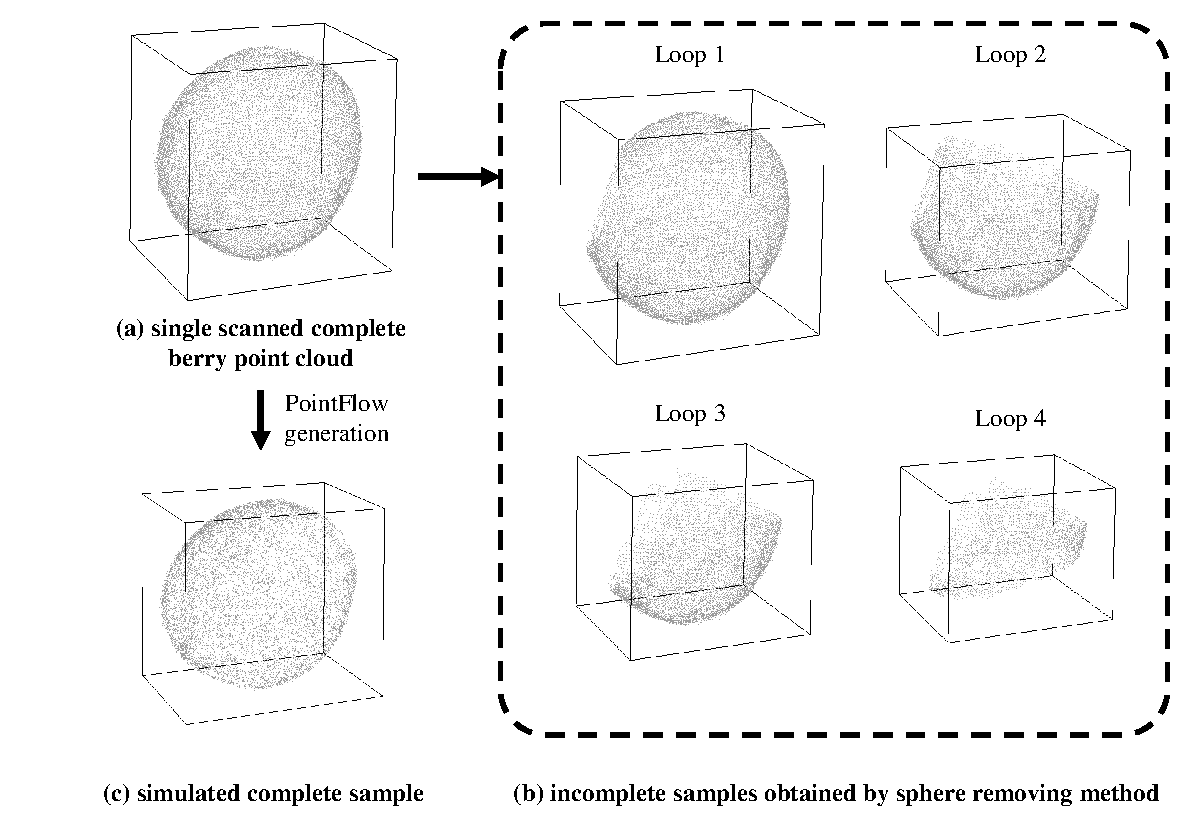
\includegraphics[width=1\textwidth]{figures/Figure9.pdf}
    \caption{\replaced[id=R2]{Workflow of automatic paired training dataset generation}{Example of dataset composition} for the \deleted[id=R2]{self-supervised training-based method of the} berry point cloud completion network.}
\end{figure}

%%%%%%%%%%%%%%%%%%%%%%%%%%%%%%%%%%%%%%%%%%%%%%%%%%%%%%%%%%%%%%%
\begin{reviewercomment}
    Table 3 results: Was the same dataset used to assess the other algorithms, or were those metrics taken from their original studies?
\end{reviewercomment}

\response{
    We appreciate the reviewer's attention to experimental rigor. 
    To ensure fair comparison, all the comparing methods were conducted on our grape dataset under the same conditions.
    We have added this clarification to the results part.
}

\manuscript{
    GrapeCPNet achieves the best results under the self-supervised training method in both the training phase and the application phase, better than the comparative algorithms \added[id=R2]{under the same condition of our grape dataset}. 
}


%%%%%%%%%%%%%%%%%%%%%%%%%%%%%%%%%%%%%%%%%%%%%%%%%%%%%%%%%%%%%%%
\begin{reviewercomment}
    Occlusion threshold: Is there a berry-occlusion threshold? 
    For example, if less than 50\% of a berry is visible, is it included? How are barely visible berries handled?
\end{reviewercomment}

\response{
    We thank the reviewer for this insightful question regarding occlusion handling. 
    Our approach was designed specifically to address challenging occlusion scenarios.

    We intentionally avoided setting visibility thresholds (e.g., 50\% cutoff) to maintain the applicable of proposed method.
    As shown in Fig.~\ref{fig:raw12}b, after removing 4 sphere regions, the incomplete berry for network training can achieved nearly around 75\% occlusion. 
    Thus, the GrapeCPNet is able to learn serever occlusions for barely visible berries.

    However, we must also admit that when severely obscured, only partial information can be seen. 
    The more obscured it is, the less information it provides. 
    Therefore, errors inevitably increase when the berry is not in a regular shape.
    As stated in the discussion part, we planed to taking prior knowledge of berry geometry to further improve the quality of completion.
}

\manuscript{
    We found that GrapeCPNet performed a little bit worse in the case of strange berry shapes, such as drop-shaped \added[id=R2]{berries, particularly when berries were sereverly occluded}.
    We subsequently consider utilizing the prior knowledge of berry geometry to achieve more detailed morphological feature extraction and representation to improve the quality of completion. 
}


%%%%%%%%%%%%%%%%%%%%%%%%%%%%%%%%%%%%%%%%%%%%%%%%%%%%%%%%%%%%%%%
\begin{reviewercomment}
    Limitations \& future directions: How will the  model perform on wine grapes. Wine grapes accounts for ~60\% of US grape  production; clusters are denser, and berries are smaller than in table grapes.
\end{reviewercomment}

\response{
    We appreciate the reviewer's insightful comment regarding wine grapes, which indeed represent a major segment of grape production. 
    In our current study, we just focused on table grape varieties commonly found in Chinese markets.
    Although they covered a wide range of cluster densities (from sparse to very dense) and berry sizes (20-35 cm axis length, as shown in Table~\ref{tbl:1} and Figure~\ref{fig:raw17}), 
    we acknowledge that wine grapes typically have smaller berry sizes lower than 13-15 mm \citep{manso_wine_2021,melo_berry_2015}, these small sizes were not included in our dataset.

    From a deep learning perspective, our model architecture should be capable of handling smaller wine grapes if provided with appropriate training data, as the fundamental detection principles remain similar regardless of grape variety. 
    Nevertheless, we agree that future work should specifically address wine grape detection through collaboration with U.S. researchers to: 
    (1) collect wine grape datasets, and 
    (2) evaluate whether models trained on table grapes can generalize well to the smaller wine grape berries without additional training.

    We have added the previous points to the discussion parts.
}

\manuscript{
    \added[id=R2]{
        This study has another limitation: it focuses only on four table grapes, which are currently common and available in Chinese markets.
        Although we examined a wide range of cluster densities (from sparse to very dense) and berry sizes (20-35 mm axis length, as shown in Table~\ref{tbl:1} and Figure~\ref{fig:raw17}),
        the study did not include wine grapes, which account for over 60\% of U.S. grape production and typically have smaller berries and denser clusters.
        As \citet{manso_wine_2021,melo_berry_2015} report, wine grape berries are often smaller than 13-15 mm, a size range not covered in our dataset.
        From a deep learning perspective, our model architecture should be able to detect smaller wine grapes with appropriate training data, as the basic detection principles are similar across grape varieties.
        Future work should involve collaboration with U.S. researchers to collect wine grape datasets and assess whether models trained on table grapes can generalize well to smaller wine grape berries without additional training.
    }

    \added[id=R1]{
        The design philosophy focuses on ensuring input quality and assigning specialized networks to their respective tasks, which provides the most efficient approach. 
    }
}



% \phantom{\cite{}} % 添加一个不可见的伪引用, 不会显示但能满足BibTeX要求避免无引用时报错
\bibliographystyle{elsarticle-harv}
% \renewcommand{\bibsection}{} % 隐藏reference标题,如果需要则注释掉这一行
\bibliography{references}

\includepdf[pages=-]{out/main.pdf} % 添加整个 PDF

\end{document}

% The copy-paste templates
\begin{verbatim}

    %%%%%%%%%%%%%%%%%%%%%%%%%%%%%%%%%%%%%%%%%%%%%%%%%%%%%%%%%%%%%%%
    \begin{reviewercomment}
        ...
    \end{reviewercomment}
    
    \response{
        ...
    }
    
    \manuscript{
        ...
    }
    
\end{verbatim}